\documentclass[11pt,psfig]{article}
\usepackage{epsfig}
\usepackage{times}
\usepackage{amssymb}
\usepackage{float}

\newcount\refno\refno=1
\def\ref{\the\refno \global\advance\refno by 1}
\def\ux{\underline{x}}
\def\uw{\underline{w}}
\def\bw{\underline{w}}
\def\ut{\underline{\theta}}
\def\umu{\underline{\mu}} 
\def\bmu{\underline{\mu}} 
\def\be{p_e^*}
\newcount\eqnumber\eqnumber=1
\def\eq{\the \eqnumber \global\advance\eqnumber by 1}
\def\eqs{\eq}
\def\eqn{\eqno(\eq)}

 \pagestyle{empty}
\def\baselinestretch{1.1}
\topmargin1in \headsep0.3in
\topmargin0in \oddsidemargin0in \textwidth6.5in \textheight8.5in
\begin{document}
\setlength{\parskip}{1.2ex plus0.3ex minus 0.3ex}


\thispagestyle{empty} \pagestyle{myheadings} \markright{Homework
4: CS 216, Image Understanding: Spring 2014}



\title{CS 216 Homework 4}
\author{Zachary DeStefano, 15247592}
\date{Due Date: May 23, 2014}

\maketitle

\vfill\eject

\newpage

\section*{Single Scale Detector Output}

\subsection*{Output for test1.jpg}

\begin{figure}[H]
\centering
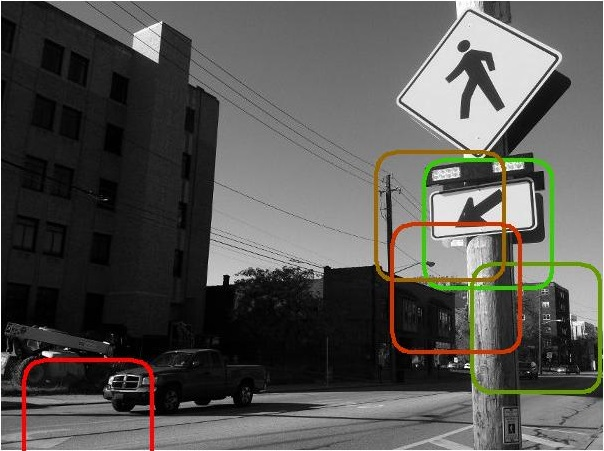
\includegraphics[height=3in]{prob5_a1plot1.jpg}
\caption{Detector Output with single positive template}
\end{figure}

\begin{figure}[H]
\centering
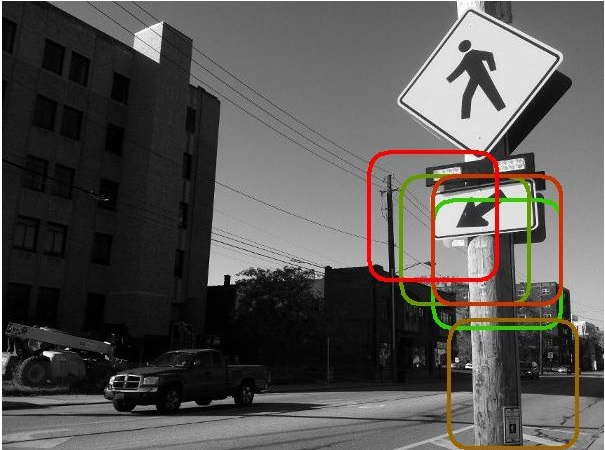
\includegraphics[height=3in]{prob5_a2plot1.jpg}
\caption{Detector Output with 5 positive templates}
\end{figure}

\begin{figure}[H]
\centering
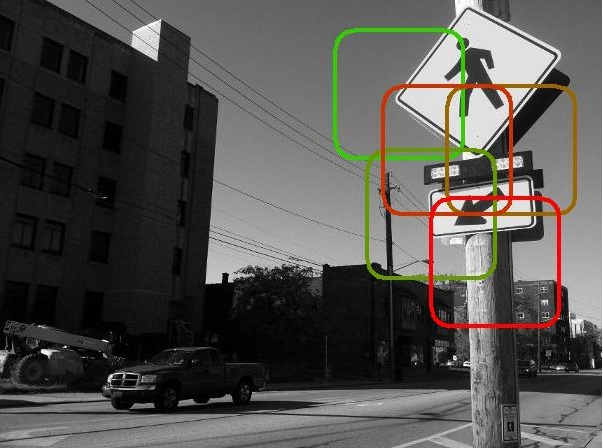
\includegraphics[height=3in]{prob5_a3plot1.jpg}
\caption{Detector Output with 5 positive templates and 100 negative templates}
\end{figure}

\subsection*{Output for test4.jpg}

\begin{figure}[H]
\centering
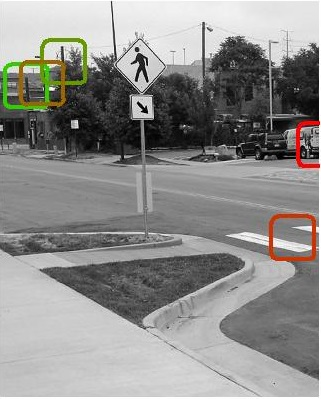
\includegraphics[height=3in]{prob5_a1plot2.jpg}
\caption{Detector Output with single positive template}
\end{figure}

\begin{figure}[H]
\centering
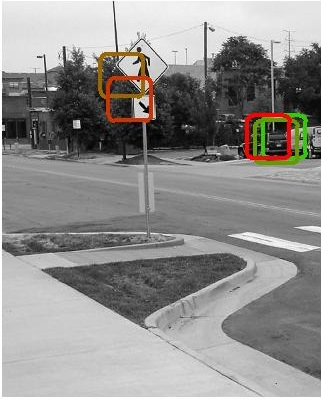
\includegraphics[height=3in]{prob5_a2plot2.jpg}
\caption{Detector Output with 5 positive templates}
\end{figure}

\begin{figure}[H]
\centering
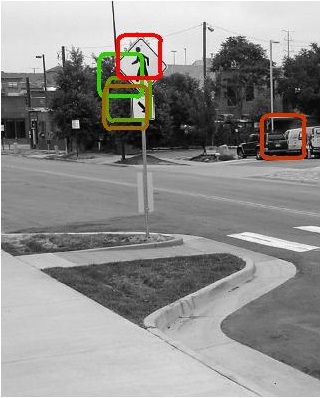
\includegraphics[height=3in]{prob5_a3plot2.jpg}
\caption{Detector Output with 5 positive templates and 100 negative templates}
\end{figure}

\section*{Multiscale Detector Output}

\subsection*{Final Output for test images}

\begin{figure}[H]
\centering
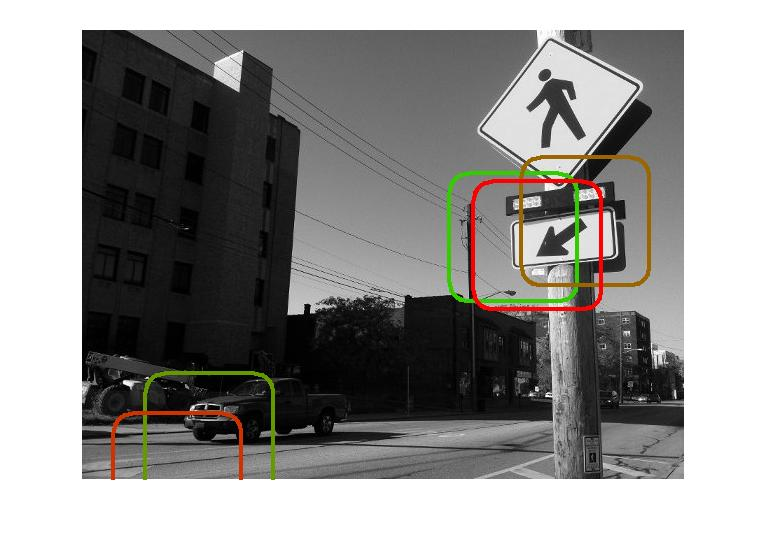
\includegraphics[height=3in]{prob5b_plot1.jpg}
\caption{Final multi scale detector output for test1.jpg}
\end{figure}

\begin{figure}[H]
\centering
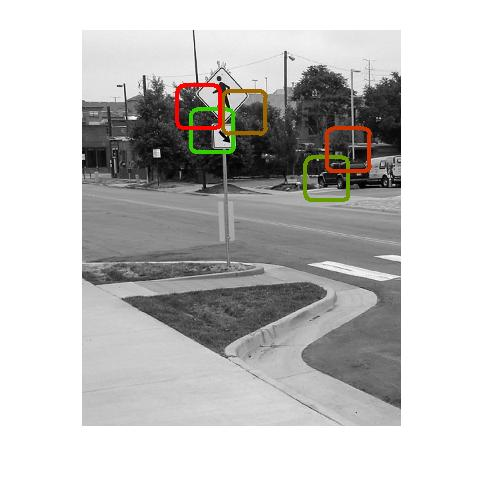
\includegraphics[height=3in]{prob5b_plot2.jpg}
\caption{Final multi scale detector output for test4.jpg}
\end{figure}


\end{document}








